\begin{figure*}[hbtp]
  \centering
  \subfigure[Initial graph]{
    \label{fig:about-frontier-01}
    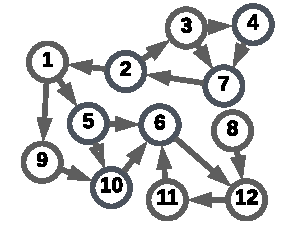
\includegraphics[width=0.23\linewidth]{out/about-frontier-01.pdf}
  }
  \subfigure[Marking affected (initial)]{
    \label{fig:about-frontier-02}
    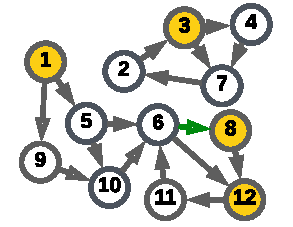
\includegraphics[width=0.23\linewidth]{out/about-frontier-02.pdf}
  }
  \subfigure[After first iteration]{
    \label{fig:about-frontier-03}
    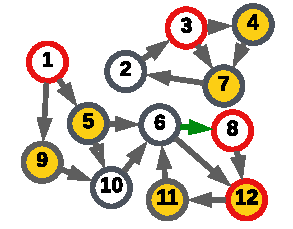
\includegraphics[width=0.23\linewidth]{out/about-frontier-03.pdf}
  }
  \subfigure[After second iteration]{
    \label{fig:about-frontier-04}
    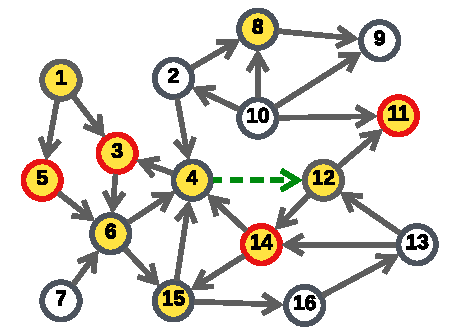
\includegraphics[width=0.23\linewidth]{out/about-frontier-04.pdf}
  } \\[-2ex]
  \caption{An example showcasing our improved \textit{Dynamic Frontier} approach. The initial graph has $12$ vertices and $16$ edges. The graph is updated with an edge insertion $(6, 8)$ and an edge deletion $(2, 1)$. Consequently, the outgoing neighbors of vertices $2$ and $6$ (i.e., vertices $1$, $3$, $8$, and $12$) are marked as affected (highlighted in yellow). In the first iteration, when computing the ranks of these affected vertices, it is observed that the relative change in rank of vertices $1$, $3$, $8$, and $12$ exceeds the frontier tolerance $\tau_f$ (indicated with a red border). Therefore, their outgoing neighbors (i.e., vertices $4$, $5$, $7$, $9$, $11$, and $12$) are also marked as affected. Vertices $1$, $3$, and $8$ are subsequently no longer marked as affected due to their relative rank change falling below the prune tolerance $\tau_p$. In the second iteration, the relative rank change of vertices $5$, $9$, $11$, and $12$ surpasses the frontier tolerance $\tau_f$, resulting in their outgoing neighbors (i.e., vertices $6$, $10$, and $11$) being marked as affected. Additionally, vertices $4$, $5$, $7$, $9$, and $12$ are no longer marked as affected as their relative rank change falls below prune tolerance $\tau_p$. In the following iteration, the rankings of affected vertices are updated once more. If the rank change of each vertex falls within the iteration tolerance $\tau$, indicating convergence, the algorithm terminates.}
  \label{fig:about-frontier}
\end{figure*}

\ignore{An example illustrating our improved \textit{Dynamic Frontier (DF)} approach. The initial graph has $12$ vertices and $16$ edges. The graph is updated with an edge insertion $(6, 8)$ and an edge deletion $(2, 1)$. Consequently, the outgoing neighbors of vertices $2$ and $6$ (i.e., vertices $1$, $3$, $8$, and $12$) are marked as affected (highlighted in yellow). In the first iteration, when computing the ranks of these affected vertices, it is observed that the change in rank of vertices $1$, $3$, $8$, and $12$ exceeds the frontier tolerance $\tau_f$ (indicated with a red border). Therefore, their outgoing neighbors (i.e., vertices $4$, $5$, $7$, $9$, $11$, and $12$) are also marked as affected. Vertices $1$, $3$, and $8$ are no longer marked as affected as the change in their rank is below the prune tolerance $\tau_p$. In the second iteration, the change in rank of vertices $5$, $9$, $11$, and $12$ exceeds the frontier tolerance $\tau_f$. Therefore, their outgoing neighbors (i.e., vertices $6$, $10$, and $11$) are marked as affected. Again, vertices $4$, $5$, $7$, $9$, $12$ are no longer marked as affected, as their change in rank falls below prune tolerance $\tau_p$. In the subsequent iteration, the ranks of affected vertices are again updated. If the change in rank of every vertex is within iteration tolerance $\tau$, the ranks of vertices have converged, and the algorithm terminates.}
